\documentclass[xcolor ={table,usenames,dvipsnames}]{beamer}
\usepackage[italian]{babel}
\usepackage{color}
\usepackage{txfonts}
\PassOptionsToPackage{dvipsnames}{xcolor}
\title{Anomaly detection using K-means}
\author{Author: Tommaso Puccetti}
\institute{Universit\`a  degli Studi di Firenze}
\date{21/12/2018}
%\usepackage{sansmathaccent}
\usetheme{Berlin} 
\useinnertheme{rounded}
\useoutertheme{miniframes} 
\setbeamercovered{dynamic}
\theoremstyle{definition}
\newtheorem{definizione}{Definizione}
\usepackage{tikz}
\usetikzlibrary{arrows}
\usepackage{subfigure}
\usepackage[procnames]{listings}
\usepackage{color}

\definecolor{keywords}{RGB}{255,0,90}
\definecolor{comments}{RGB}{0,0,113}
\definecolor{red}{RGB}{160,0,0}
\definecolor{green}{RGB}{0,150,0}

\lstset{language=Python, 
	backgroundcolor=\color{yellow},
	basicstyle=\fontsize{2}{4}\selectfont\ttfamily\scriptsize, 
	keywordstyle=\color{keywords},
	commentstyle=\color{comments},
	stringstyle=\color{green},
	showstringspaces=false,
	identifierstyle=\color{black},
	procnamekeys={def,class},
}

\begin{document}
	
	\begin{frame}
		\maketitle
	\end{frame}

	\begin{frame}
		\frametitle{Clustering: basics}
			Clustering analysis \textit{is a collection of statistical methods that can be used to assign units
				to groups, where group members share some characteristic}.  
			
			\begin{itemize}
				\item \textbf{data reduction}: reduce data that are homogeneous (similar)
				\item \textbf{find “natural clusters”} and describe their unknown properties
				\item \textbf{find} useful and suitable \textbf{groupings}
				\item \textbf{find} unusual data objects (i.e. outlier detection).
			\end{itemize}
		
			The aim is to find a way of \textbf{grouping statistical units} (or variables) in a data
			set in such a way that:
			\textbf{units are similar within groups and dissimilar among groups}.
	\end{frame}

	\begin{frame}
		\frametitle{Clustering algorithm}
			The essentials steps for a clustering algorithm are the following:
			
			\begin{enumerate}
				\item Define a \textbf{metric} to evaluate distances between units;
				\item Define an \textbf{algorithm} to form groups. \\
			\end{enumerate}
			
			A \textbf{grouping} algorithm can be:
			\begin{itemize}
				\item \textbf{Hierarchical}
				\item \textbf{Non Hierarchical}
			\end{itemize}	
	\end{frame}

	\begin{frame}
		\frametitle{Non-hierarchical clustering: K-means}
		K-means clustering is one of the simplest and popular unsupervised machine learning algorithms. The aim is to find a partition of the dataset into a set of K clusters that optimizes the chosen partitioning criterion.
		
		\begin{enumerate}
			\item choose K points at random as cluster centers
			(centroids);
			\item assign each unit to its closest centroid,
			using an opportune distance measure (usually Euclidean or Manhattan);
			\item calculate the centroid of each cluster and use it as
			the new cluster center;
			\item go back to step 2, stop when cluster centers
			do not change any more.
		\end{enumerate}
	\end{frame}

	\begin{frame}[fragile]
		\frametitle{K-means: implementation (1)}
		\begin{itemize}
			\item First of all the algorithm choose K random centroid.
			\begin{lstlisting}
z = self.rng.permutation(len(X))[:self.k]
X = np.array(X, dtype= "float64")
centers = X[z]
			\end{lstlisting}
			
		\end{itemize}
	\end{frame}

	\begin{frame}[fragile]
		\frametitle{K-means: implementation (2)}
		\begin{itemize}
			\item The second step of the fit() method is to \textbf{calculate the} \textbf{Euclidean distance} between all the dataset points in respect to the K centroids. The distances are used to assign all the points to the nearest cluster, using K labels. 
			$$d(x,y) = \sqrt[2]{\sum_{i=0}^n (x_{i} - y_{i})^{2}} $$
			\begin{lstlisting}
for i in range(self.k):
	distances[:,i] = np.linalg.norm(X - centers[i],
		axis=1)	
			
	labels= np.argmin(distances, axis = 1)
			\end{lstlisting}
		\end{itemize}
		
	\end{frame}

	\begin{frame}[fragile]
		\frametitle{K-means: implementation (3)}	
		\begin{itemize}
			\item For each cluster the algorithm \textbf{calculates the new centroid} as the mean of the points assigned to them:
			
			\begin{lstlisting}
for i in range(self.k):
	if(i in labels):
		new_centers = X[labels == i].mean(0)
		center_temp.append(new_centers)
	else:
		center_temp.append(self.farthest(X, 
			distances, labels))	
		new_centers = np.array(center_temp,
			dtype= "float64")
			\end{lstlisting}
		\end{itemize}
	\end{frame}

	\begin{frame}[fragile]
		\frametitle{K-means: implementation (4)}
		\item Repeats from point 2 to point 3 until the new centroids are equal to the centroids from the previous step.
		\begin{lstlisting}
if np.all(centers == new_centers):
	break
		
	centers = new_centers
		\end{lstlisting}
	\end{frame}

	\begin{frame}[fragile]
		\frametitle{K-means: example}
		The \textbf{\textit{kmeans\_sk.py}} file contains an example of usage for the algorithm. The artificial data presents 4 distinct points aggregates. Using the \textbf{\textit{fit()}} method with $K = 4$ the algorithm, as we expected, identifies the 4 aggregates of points as 4 clusters.
		
		INSERIRE IMMAGINI ESEMPIO AFFIANCATE
	\end{frame}

	\begin{frame}[fragile]
		\frametitle{Anomaly detection using K-means}
		K-means algorithm can be used to spot anomalies given the normal behaviour.
			\begin{figure}[]
			\centering
			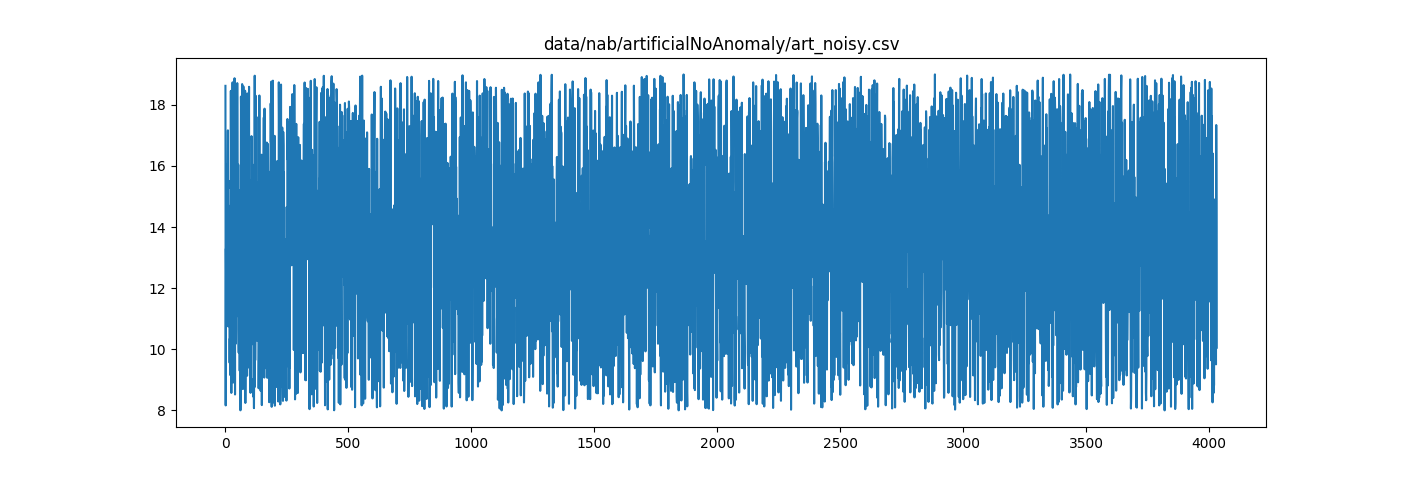
\includegraphics[scale=0.15]{img/normalbe.png}
		\end{figure}
		
		\begin{figure}[]
			\centering
			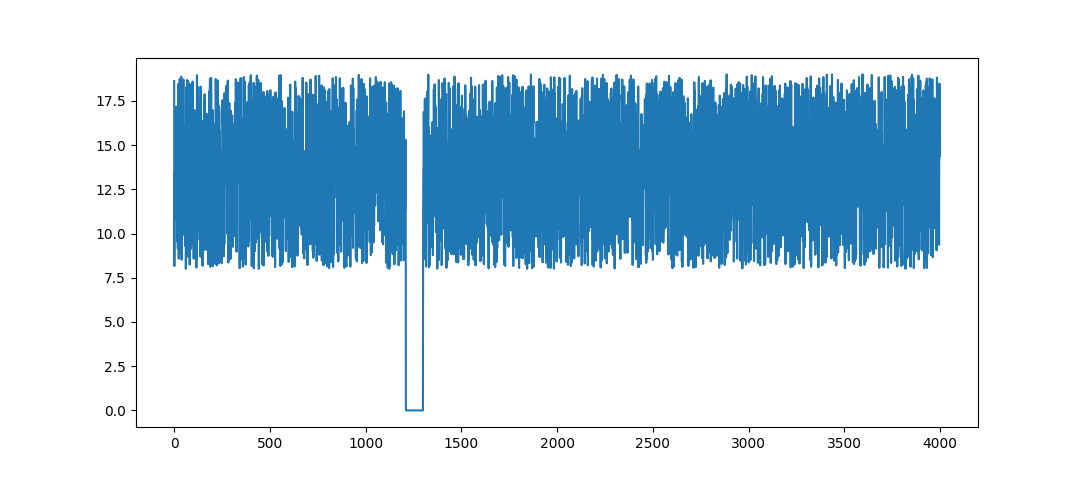
\includegraphics[scale=0.20]{img/anomaly.png}
		\end{figure}
	
	\end{frame}

	\begin{frame}
		\frametitle{Anomaly detection using K-means: implementation (1)}
		The idea is the following:
		\begin{itemize}
			\item split the waweform into \textbf{\textit{n}} segments of length \textbf{\textit{l}}: every segment is considered a statistical unit;
			\item apply the K-means algorithm over the l-dimension points obtained (segments). The results are K cluster's \textit{centroids};
			\item a centroid is a segments itself that can be used to reconstruct the original waweform: for every segments the nearest centroid is used to approximate the current;
		\end{itemize}
	\end{frame}

	\begin{frame}
		\frametitle{Anomaly detection using K-means: implementation (2)}
		\begin{itemize}
			\item once obtained a recostructed waweform using only centroids, we can subtract it from the original: the result is also a waweform that rapresents the noise signal between the two;
			\item the last step is to use a treshold value to detect where the error between the original and the reconstructed waweforms is anomalous in respect to the noise obtained. 
		\end{itemize}
	\end{frame}

	\begin{frame}
		\frametitle{Segmentation}
		INSERIRE IMMAGINE FINESTRE
		
	\end{frame}

	\begin{frame}[fragile]
		\frametitle{Segmentation}
		
		The segmentation is done using the \textit{segmentation()} function implemented in the K-means class.
		
		\begin{lstlisting}
segment_len = 32
slide_len = 16
km = skmeans.K_means(30)
segments = km.segmentation(train_array, segment_len, slide_len)
		\end{lstlisting}
		
		The output would be a Numpy's array containing the segments obtained.
			 
		\end{frame}

	\begin{frame}[fragile]
		\frametitle{Calculate centroids}
		\begin{lstlisting}
		centr = km.fit(segments)
		learn_utils.plot_waves(centr, step=3)
		\end{lstlisting}	
		The output would be a Numpy's array containing K centroids of the dataset. The picture below shows some of the normal waweform obtained.
		
		\begin{figure}[h!]
			\centering
			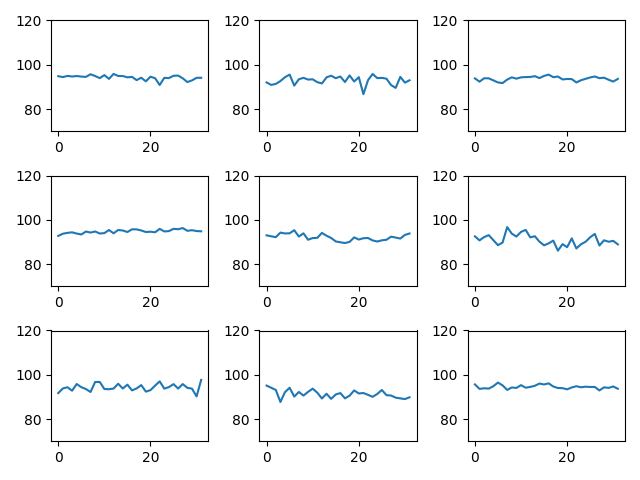
\includegraphics[scale=0.35]{img/centroids.png}
		\end{figure}
	\end{frame}

	
	\begin{frame}[fragile]
		\frametitle{Reconstruction (1)}
		Once obtained the centroids we can use them to reconstruct the original waweform. First of all we have to apply again the segmentation process, this time over the entire dataset. 
		
				
		\begin{lstlisting}
segments = km.segmentation(dataset_array, segment_len, slide_len)
lab = km.predict(centr, segments)
		\end{lstlisting}  
	\end{frame}

	\begin{frame}[fragile]
		\frametitle{Reconstruction (2)}
		Then the \textbf{\textit{predict()}} function is used to find, for all the segments obtained, the nearest centroid. The output would be an array wich store in the n-th position a label referring to the nearest centroid for the n-th segment.
		
			\begin{lstlisting}
Predicted Labels
[12 27 3 14 23 22 27 16 12 26 12 19 4 5 7 6 6 6 28 10 9 1 10 4
29 16 6 21 20 15 13 9 24 7 12 2 17 17 11 1 23 9 10 9 11 11 10 6
6 8 0 8 9 9 1 11 0 23 0 21 26 27 6 8 24 23 25 25 10 23 25 8
9 10 25 1 11 10 5 23 24 0 10 8 9 10 23 23 0 23 23 18 10 10 7 23
                     ................... 
20 21 26 21 26 26 21 21 26 21 21 26 20 27  6  7 27 12 27 14  6 
21 21 15 21 13 13 27 6 10 0 23 9 0 12 21 12 12 20 20 27 12 27 12 
27 21 21 20 23 23 9 0 9 10 10 8 9]
		\end{lstlisting}
	\end{frame}

	\begin{frame}[fragile]
		\frametitle{Reconstruction (3)}
		Finally the reconstruction algorithm is used to obtain the whole waweform. 
		
		\begin{lstlisting}
noise = detection.reconstruction(dataset_array, segments, lab, 
centr, slide_len, segment_len)
		\end{lstlisting}
		The noise obtained as output is ploted along with the original and the reconstructed waweform.
		
		\begin{figure}[h!]
			\centering
			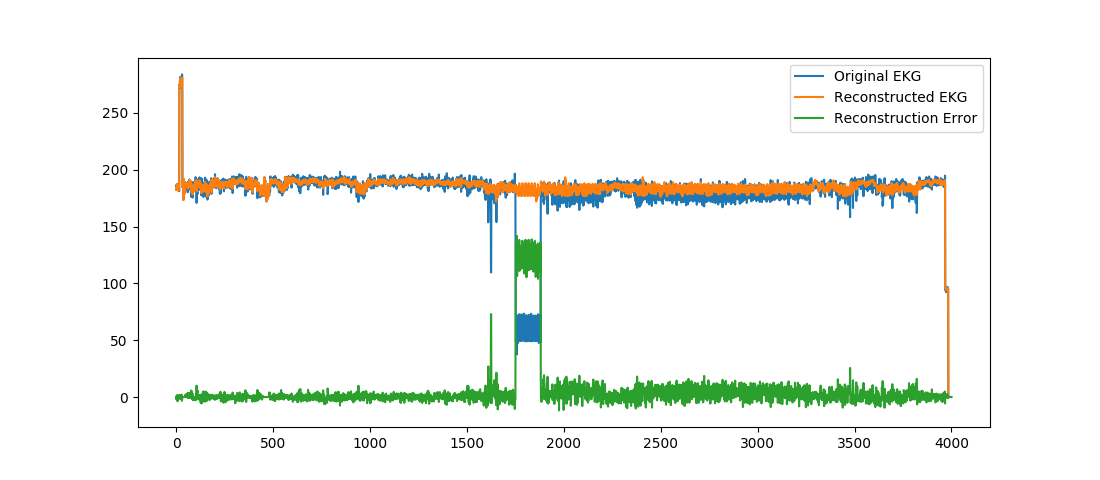
\includegraphics[scale=0.3]{img/noise.png}
		\end{figure}
	\end{frame}

	
	
\end{document}